% ARCHIVED single-run IEEE-format draft (numbers superseded). The current manuscript is main_acm.tex.
\documentclass[lettersize,journal]{IEEEtran}

\usepackage{cite}
\usepackage{amsmath,amssymb,amsfonts}
\usepackage{algorithm}
\usepackage{algorithmic}
\usepackage{array}
\usepackage{textcomp}
\usepackage{stfloats}
\usepackage{url}
\usepackage{graphicx}
\usepackage{bm}
\usepackage{makecell}
\usepackage{pifont}
\usepackage{booktabs}
\usepackage{multirow}
\usepackage{tikz}
\usetikzlibrary{arrows.meta,positioning,fit,shapes.geometric,calc}
\usepackage[hidelinks]{hyperref}

\hyphenation{op-tical net-works semi-conduc-tor IEEE-Xplore}

\newcommand{\cmark}{\ding{51}}
\newcommand{\xmark}{\ding{55}}
% Shared TikZ styles for the framework diagrams (original vector drawings)
\tikzset{
  agent/.style={draw, rounded corners=2pt, fill=blue!6, align=center, font=\footnotesize, minimum height=8mm, inner sep=3pt},
  wm/.style={draw, rounded corners=2pt, fill=orange!10, align=center, font=\footnotesize, inner sep=4pt},
  op/.style={draw, fill=white, align=center, font=\scriptsize, inner sep=2.5pt, rounded corners=1pt},
  gate/.style={draw, diamond, aspect=2.2, fill=green!8, align=center, font=\scriptsize, inner sep=1pt},
  st/.style={draw, circle, fill=white, font=\scriptsize, inner sep=1.2pt, minimum size=6.5mm},
  flow/.style={-{Latex[length=1.8mm]}, semithick},
  fb/.style={-{Latex[length=1.8mm]}, semithick, dashed, red!65!black},
  lbl/.style={font=\scriptsize, align=center, fill=white, inner sep=1pt},
  panel/.style={draw=gray!60, rounded corners=3pt, inner sep=6pt},
  ttl/.style={font=\footnotesize\bfseries},
}

\makeatletter
\newcommand{\tabinput}[1]{\@@input #1 }
\makeatother

% Original title: "How Can World Models Fit in Cyber-Physical AI Multi-Agent Reasoning Systems?"
\title{Do World Models Help Multi-Agent LLM Reasoning? A Controlled Study of State-Centric Coordination}

\author{
Yu~Wang and Vijay~K.~Madisetti,~\IEEEmembership{Fellow,~IEEE}%
\thanks{Yu Wang is with the College of Computing, Georgia Institute of Technology, Atlanta, GA 30332 USA (e-mail: ywang4704@gatech.edu).}
\thanks{Vijay K. Madisetti is with the School of Cybersecurity and Privacy, Georgia Institute of Technology, Atlanta, GA 30332 USA (e-mail: vkm@gatech.edu).}
}

\markboth{Preprint}%
{Wang \MakeLowercase{\textit{et al.}}: Do World Models Help Multi-Agent LLM Reasoning?}

\begin{document}

\maketitle

\begin{abstract}
World models---explicit representations of state, transitions, and predicted outcomes---have been proposed as a way to make multi-agent systems built on large language models (LLMs) more reliable than systems that coordinate through unstructured conversation.
We study this proposal in a controlled setting. We equip a reviewer-style multi-agent pipeline (author, independent reviewers, meta-reviewer) with a lightweight symbolic world model that stores every candidate solution as an explicit state, validates state transitions, estimates a trajectory-level risk from the reviews, and, in its \emph{centralized} form, gates the acceptance of a candidate independently of any single agent's verdict; a \emph{peer-to-peer} form keeps local state replicas and leaves acceptance to the agents.
All configurations and six external baselines are evaluated with up to four backbone LLMs on identical questions from eight reasoning benchmarks, with paired statistical tests.
Three findings emerge.
First, without a state-level gate the review process almost never changes the outcome: the meta-reviewer accepts 81--99\% of incorrect drafts in the first round, and message-based and peer-to-peer coordination are statistically indistinguishable.
Second, the centralized gate does intervene, but its benefit depends on the backbone: it yields a net within-run gain of 4.3 accuracy points on one model, 1.3 on two others, and none on the fourth, at 1.6--4.2 times the token cost. On the three more recent models the gate blocks most incorrect drafts but also most correct ones, and blocked incorrect drafts are repaired in only 5--34\% of cases.
Third, a coordination-uncertainty index computed from reviewer disagreement does not reliably predict which coordination mode is preferable; the sign of the association differs across backbones.
Across all methods, including debate-style baselines, multi-agent collaboration improves on a single chain-of-thought call by at most about two points on these benchmarks.
We conclude that the bottleneck of reviewer-style multi-agent reasoning is not the representation of state but the discriminative power of acceptance decisions and the ability of the author agent to revise, and we report an exploratory variant that targets these two points.
\end{abstract}

\begin{IEEEkeywords}
world models, multi-agent reasoning, large language models, state-centric coordination, acceptance gating, coordination uncertainty
\end{IEEEkeywords}

\section{Introduction}

\IEEEPARstart{L}{arge} language models (LLMs) reason more reliably when their outputs are produced with structured prompting such as chain-of-thought and self-consistency~\cite{wei2022chain,wang2023selfconsistency}, and a large literature now attempts to go further by letting several LLM agents debate, review, or collaborate~\cite{du2024improving,liang2024mad,chen2024reconcile,qian2024chatdev,hong2024metagpt,wang2025mars}.
In almost all of these systems coordination is mediated by natural-language messages: the evolving state of the solution---which candidate is under consideration, how it was obtained, how reliable it is believed to be---is implicit in the conversation history.

World models offer an alternative view. In reinforcement learning a world model represents environment states and transitions explicitly so that an agent can evaluate trajectories before committing to them~\cite{ha2018recurrent,hafner2020dream}, and related ideas have entered LLM agents through explicit memories, environment feedback, and search over reasoning states~\cite{park2023generative,wang2024voyager,yao2023react,hao2023rap}.
It is therefore natural to ask whether a multi-agent reasoning system benefits from coordinating through an explicit, validated task state rather than through the raw message stream, and whether that state should be owned centrally or replicated across agents.

This paper examines the question empirically. We formulate reviewer-style multi-agent reasoning as a state-transition process and implement a deliberately simple world model for it: a symbolic store of states with rule-based transition validation and a rule-based trajectory-risk estimate (Fig.~\ref{fig:concept}).
We study two ways of using it.
In \emph{centralized} coordination one world model is the single holder of state and gates acceptance: a candidate is returned only if the reviewers' consensus, their reliability, and the trajectory risk satisfy a state-level test, regardless of the meta-reviewer's verdict.
In \emph{peer-to-peer} coordination each agent keeps a local replica, state summaries travel inside messages, and acceptance is left to the agents.
We also define a Coordination Uncertainty Index (CUI) from reviewer disagreement and test the hypothesis that it predicts which mode is preferable.

Our evaluation is designed to isolate the effect of the coordination mechanism. Every configuration is run on the same fixed questions of eight benchmarks with four backbone LLMs; six external baselines are re-implemented in the same pipeline; all comparisons are paired; and, because the author's first draft is logged, the effect of each mechanism can be measured \emph{within} a run as the difference between draft and final accuracy.
We address four research questions:

\begin{itemize}
    \item \textbf{RQ1:} Does world-model--guided coordination improve accuracy over message-based coordination, and at what cost?
    \item \textbf{RQ2:} Through which mechanism does it act, and where does it fail?
    \item \textbf{RQ3:} Can task uncertainty, measured by the CUI, predict which coordination mode is preferable?
    \item \textbf{RQ4:} How do reviewer-style configurations compare with recent multi-agent reasoning methods under identical conditions?
\end{itemize}

The answers are more sobering than the premise suggests, and we report them as they are:

\begin{itemize}
    \item \textbf{C1 (framework).} We give a complete specification of a state-centric coordination framework for multi-agent LLM reasoning, with explicit state composition, transition, validation, risk, and acceptance rules, in a centralized and a peer-to-peer variant (Section~\ref{sec:method}).
    \item \textbf{C2 (controlled evidence).} On 1{,}592 paired questions across four backbones, peer-to-peer coordination is indistinguishable from the message-based pipeline, and centralized coordination improves accuracy significantly on one backbone only, at up to four times the token cost (Section~\ref{sec:main_results}).
    \item \textbf{C3 (diagnosis).} We identify why: ungated pipelines accept 81--99\% of incorrect drafts; on the three more recent backbones the state-level gate blocks 73--81\% of incorrect drafts but also 56--60\% of correct ones; and a blocked incorrect draft is subsequently repaired in only 5--34\% of cases, least often with the strongest backbone (Section~\ref{sec:gate_results}).
    \item \textbf{C4 (negative result on adaptivity).} The CUI does not reliably predict the preferable mode: its correlation with the peer--centralized accuracy gap is positive on two backbones, negative on one, and absent on one, and no CUI threshold yields a policy that consistently beats the better fixed mode (Section~\ref{sec:cui_results}).
    \item \textbf{C5 (context).} Under identical conditions, six external baselines and all reviewer-style configurations lie within a few points of a single chain-of-thought call (Section~\ref{sec:baseline_results}).
\end{itemize}

\begin{figure*}[!t]
    \centering
    \resizebox{\textwidth}{!}{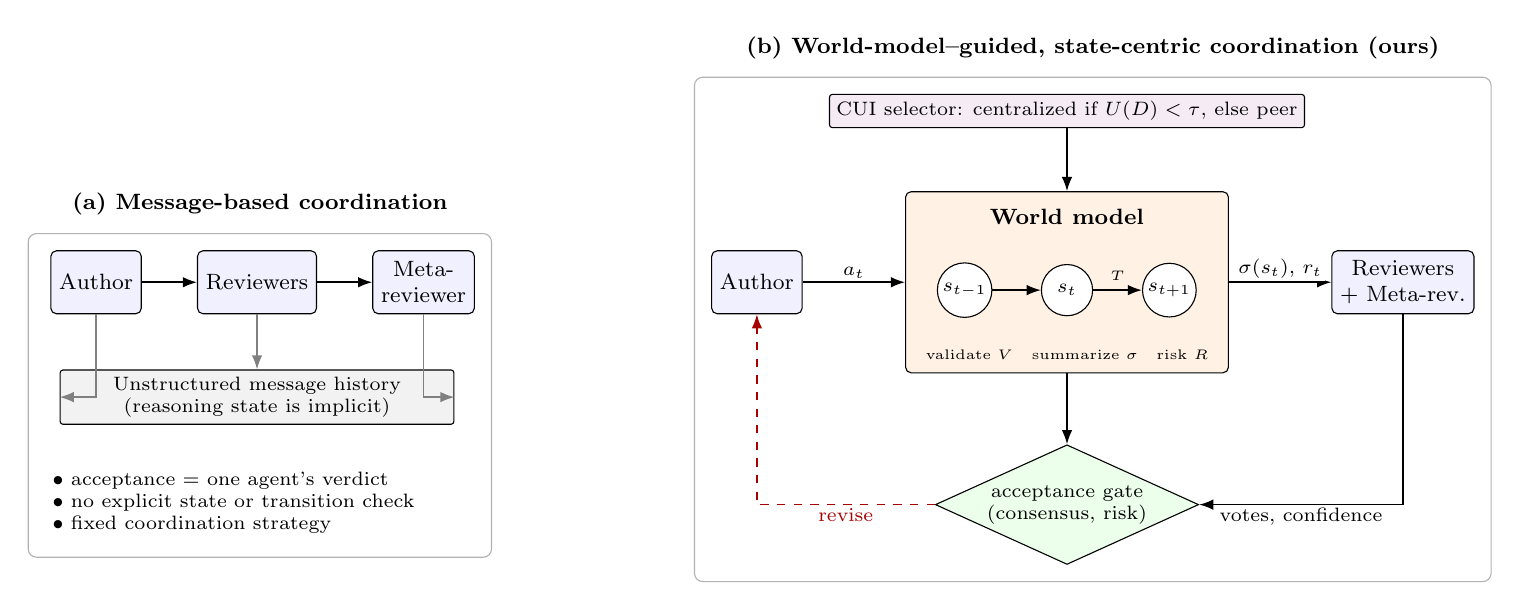
\begin{tikzpicture}[node distance=6mm and 7mm]
% ---------------- (a) message-based ----------------
\node[agent] (a1) {Author};
\node[agent, right=of a1] (r1) {Reviewers};
\node[agent, right=of r1] (m1) {Meta-\\reviewer};
\draw[flow] (a1) -- (r1);
\draw[flow] (r1) -- (m1);
\node[op, below=7mm of r1, minimum width=50mm, fill=gray!10] (hist) {Unstructured message history\\(reasoning state is implicit)};
\draw[flow, gray] (a1) |- (hist.west);
\draw[flow, gray] (r1) -- (hist);
\draw[flow, gray] (m1) |- (hist.east);
\node[op, below=5mm of hist, draw=none, text width=52mm, align=left] (n1) {%
$\bullet$ acceptance = one agent's verdict\\
$\bullet$ no explicit state or transition check\\
$\bullet$ fixed coordination strategy};
\node[panel, fit=(a1)(m1)(hist)(n1)] (pa) {};
\node[ttl, above=1mm of pa] {(a) Message-based coordination};

% ---------------- (b) state-centric ----------------
\node[agent, right=30mm of m1] (a2) {Author};
\node[wm, right=13mm of a2, minimum width=41mm, minimum height=23mm] (w) {};
\node[ttl, anchor=north] at ([yshift=-1mm]w.north) {World model};
\node[st] (s0) at ([xshift=-13mm,yshift=-1mm]w.center) {$s_{t-1}$};
\node[st] (s1) at ([yshift=-1mm]w.center) {$s_{t}$};
\node[st] (s2) at ([xshift=13mm,yshift=-1mm]w.center) {$s_{t+1}$};
\draw[flow] (s0) -- (s1);
\draw[flow] (s1) -- node[above, font=\tiny] {$T$} (s2);
\node[font=\tiny, anchor=south] at ([yshift=0.5mm]w.south) {validate $V$\quad summarize $\sigma$\quad risk $R$};
\node[agent, right=13mm of w] (r2) {Reviewers\\+ Meta-rev.};
\draw[flow] (a2) -- node[lbl, above] {$a_t$} (w);
\draw[flow] (w) -- node[lbl, above] {$\sigma(s_t)$, $r_t$} (r2);
\node[gate, below=9mm of w] (g) {acceptance gate\\(consensus, risk)};
\draw[flow] (r2) |- node[lbl, pos=0.75, below] {votes, confidence} (g);
\draw[flow] (w) -- (g);
\draw[fb] (g) -| node[lbl, pos=0.25, below] {revise} (a2);
\node[op, above=8mm of w, fill=violet!8] (cui) {CUI selector: centralized if $U(D)<\tau$, else peer};
\draw[flow] (cui) -- (w);
\node[panel, fit=(a2)(r2)(g)(cui)] (pb) {};
\node[ttl, above=1mm of pb] {(b) World-model--guided, state-centric coordination (ours)};
\end{tikzpicture}
}
    \caption{Message-based coordination (a) versus the state-centric coordination studied in this paper (b). In (b) each candidate solution is committed to a world model as an explicit state; the world model validates transitions, summarizes the state for reviewers, estimates a trajectory risk, and can gate acceptance.}
    \label{fig:concept}
\end{figure*}

\section{Related Work}

\paragraph{Multi-agent LLM reasoning.}
A growing body of work improves LLM reasoning by letting several model instances critique one another.
Multi-agent debate lets agents exchange and revise answers over several rounds~\cite{du2024improving}; MAD assigns opposing roles to two debaters and adds a judge that can end the debate~\cite{liang2024mad}; ReConcile runs a round-table discussion among diverse LLMs and aggregates their answers by confidence-weighted voting~\cite{chen2024reconcile}.
Self-refinement and reflection methods apply the same critique--revise loop within a single model~\cite{madaan2023selfrefine,shinn2023reflexion}.
Role-based systems such as ChatDev, MetaGPT, and AutoGen organize agents into specialized roles that collaborate through structured conversations~\cite{qian2024chatdev,hong2024metagpt,wu2024autogen}.
Closest to our setting, MARS organizes agents as an author, independent reviewers, and a meta-reviewer, which removes reviewer-to-reviewer communication and thereby reduces the token cost of fully connected debate~\cite{wang2025mars}.
Our framework adopts this reviewer-style role structure and uses it as the message-based baseline.

\paragraph{Role specialization, workflow optimization, and graph-structured orchestration.}
Recent systems go beyond fixed role assignments.
AgentVerse dynamically recruits a group of expert agents for each task and alternates collaborative decision making with evaluation~\cite{chen2024agentverse}; DyLAN selects and re-weights agents during inference through an agent-importance score~\cite{liu2024dylan}.
Role-specialized pipelines have also been shown to be effective beyond question answering: Zhao et al.\ combine multiple LLM agents with small models for zero-shot knowledge-graph question generation, assigning distinct sub-tasks to distinct agents~\cite{zhao2024kgqg}.
A second line of work treats the communication structure itself as the object of optimization.
MacNet arranges agents on directed acyclic graphs and studies how collaboration scales with topology~\cite{qian2025scaling}; GPTSwarm represents an agent system as a computational graph whose node prompts and edge connectivity are optimized~\cite{zhuge2024gptswarm}; AgentPrune removes redundant messages from the spatial--temporal communication graph to reduce cost~\cite{zhang2025agentprune}.
These approaches decide \emph{who} talks to \emph{whom}.
Our work is complementary: we keep the topology fixed and ask \emph{what} the agents coordinate through---an explicit, validated task state rather than the raw message stream---and whether the degree of centralization of that state should depend on task uncertainty.
An uncertainty signal such as the CUI could in principle be used as an input to topology-selection methods.

\paragraph{Memory-based agents.}
Memory mechanisms also structure the context of LLM agents and are therefore closely related to our use of explicit state.
Generative Agents store a stream of observations and retrieve from it by recency, relevance, and importance~\cite{park2023generative}; MemGPT pages information between the context window and external storage in the manner of an operating system~\cite{packer2023memgpt}; MemoryBank maintains and updates a long-term store with a forgetting mechanism~\cite{zhong2024memorybank}; Reflexion and Voyager accumulate verbal lessons and executable skills across episodes~\cite{shinn2023reflexion,wang2024voyager}; and CoALA provides a unifying taxonomy of working, episodic, semantic, and procedural memory for language agents~\cite{sumers2024coala}.
In CoALA's terms, our state store is a structured \emph{working memory} for a single task, and we do not claim a new memory architecture.
The difference lies in what the structure is used for.
Memory systems answer the question ``which past information should be placed in the context?''; their central operations are write, retrieve, and summarize, and their goal is to preserve information across long horizons.
The world model in our framework answers the question ``may this proposed step be committed, and may the current trajectory be accepted?''; its central operations are a typed transition, a validator that can reject an action before other agents see it, and a risk function over the trajectory that gates acceptance independently of any single agent's verdict.
Our state is also not persistent: it is created per query and discarded afterwards, so none of the reported gains can come from cross-task memory.
The two ideas are compatible, and combining a persistent memory with state-level validation is a natural extension.

\paragraph{World models and structured reasoning.}
World models were introduced in reinforcement learning to represent environment states and transitions and to plan by imagined rollouts~\cite{ha2018recurrent,hafner2020dream}.
In the LLM literature, RAP uses the LLM itself as a world model that predicts the next reasoning state and plans with Monte-Carlo tree search~\cite{hao2023rap}, Tree-of-Thoughts evaluates and searches over partial solutions~\cite{yao2023tree}, and ReAct and Toolformer couple reasoning with environment or tool feedback~\cite{yao2023react,schick2023toolformer}.
These methods structure the reasoning of a single agent.
Our world model is far simpler than a learned dynamics model---it is a symbolic state store with rule-based validation and risk estimation---but it is shared across agents and used for coordination: it determines what reviewers see and when a candidate is accepted.

\paragraph{Positioning.}
Table~\ref{tab:related_work} summarizes the comparison.
To our knowledge, prior multi-agent reasoning frameworks do not combine an explicit per-task state object, validation of state transitions, a trajectory-level acceptance test, and a task-dependent choice of coordination mechanism.
The table also makes the limits of our framework explicit: it has neither persistent cross-task memory nor a learned communication topology.

\begin{table*}[!t]
\caption{Positioning Against Representative Approaches (\cmark: supported; \xmark: not supported; $\circ$: partially)}
\label{tab:related_work}
\centering
\footnotesize
\setlength{\tabcolsep}{2.5pt}
\renewcommand{\arraystretch}{1.15}
\begin{tabular}{lccccccc}
\toprule
 & \makecell{Debate / MAD\\\cite{du2024improving,liang2024mad}} & \makecell{ReConcile\\\cite{chen2024reconcile}} & \makecell{MARS\\\cite{wang2025mars}} & \makecell{AgentVerse\\\cite{chen2024agentverse}} & \makecell{GPTSwarm\\\cite{zhuge2024gptswarm}} & \makecell{Memory agents\\\cite{packer2023memgpt,zhong2024memorybank}} & Ours \\
\midrule
Multi-agent critique of candidate answers & \cmark & \cmark & \cmark & \cmark & \cmark & \xmark & \cmark \\
Explicit per-task state object & \xmark & \xmark & \xmark & \xmark & \xmark & $\circ$ & \cmark \\
Validation of state transitions & \xmark & \xmark & \xmark & \xmark & \xmark & \xmark & \cmark \\
Acceptance independent of a single agent's verdict & $\circ$ & \cmark & \xmark & $\circ$ & $\circ$ & \xmark & \cmark \\
Persistent cross-task memory & \xmark & \xmark & \xmark & \xmark & \xmark & \cmark & \xmark \\
Dynamic or optimized agent topology & \xmark & \xmark & \xmark & \cmark & \cmark & \xmark & \xmark \\
Uncertainty-dependent coordination mode & \xmark & \xmark & \xmark & \xmark & \xmark & \xmark & \cmark \\
\bottomrule
\end{tabular}
\end{table*}

\section{Problem Formulation}
\label{sec:problem_formulation}

We consider a multi-agent reasoning system built on large language models (LLMs).
Given an input query \(x\), the objective is to produce a correct final answer \(y\) through a bounded number of interaction rounds among an author agent, \(k\) reviewer agents, and a meta-reviewer agent.

Existing multi-agent LLM frameworks typically represent the reasoning process implicitly, as a sequence of natural-language messages exchanged among agents~\cite{du2024improving,qian2024chatdev,hong2024metagpt,wang2025mars}.
Such message-based representations do not expose an explicit object that records which candidate solution is currently under consideration, how it was derived, and how reliable it is judged to be.
We therefore formulate multi-agent reasoning as a \emph{state-transition process} over an abstract task environment, inspired by world-model approaches to sequential decision making~\cite{ha2018recurrent,hafner2020dream}.

\paragraph{States, actions, transitions.}
Let \(s_t \in \mathcal{S}\) denote the task state after the \(t\)-th committed action, with \(s_0\) derived from the query \(x\).
An action \(a_t \in \mathcal{A}\) is a typed proposal produced by an agent (a draft or a revision of a candidate solution).
Committing an action yields a new state through a transition function
\begin{equation}
s_{t+1} = T(s_t, a_t, o_t),
\end{equation}
where \(o_t\) is an optional observation (in our setting, the index of the review round).
A reasoning \emph{trajectory} is the sequence \(\xi = (s_0, s_1, \ldots, s_H)\) with horizon \(H\).

\paragraph{Validation and risk.}
Two evaluation functions operate on states. A validator
\begin{equation}
V(s_t, a_t) \rightarrow (\mathit{ok}, \mathit{hint})
\end{equation}
decides whether a proposed action may be passed on to the reviewers, and a rollout function
\begin{equation}
R(s_t, \mathcal{F}_t) \rightarrow r_t \in [0,1]
\end{equation}
maps the current state and the reviewer feedback \(\mathcal{F}_t\) collected for it to a \emph{trajectory risk}: an estimate of how likely it is that accepting the current candidate would be a mistake.

\paragraph{Coordination as a policy.}
A coordination mechanism \(\pi\) specifies who owns the state, which information each agent sees, and under which condition a candidate is accepted.
We study two mechanisms (centralized and peer-to-peer, Section~\ref{sec:method}) and an uncertainty-dependent rule for choosing between them: for a task distribution \(D\) with coordination uncertainty \(U(D)\),
\begin{equation}
\label{eq:policy}
\pi^{*}(D) =
\begin{cases}
\text{Centralized}, & U(D) < \tau,\\
\text{Peer}, & U(D) \ge \tau,
\end{cases}
\end{equation}
where \(\tau\) is a threshold.
Eq.~\eqref{eq:policy} is a hypothesis to be tested empirically, not an optimality result; Section~\ref{sec:cui} defines \(U(D)\) and Section~\ref{sec:cui_results} examines how well the rule holds.

\section{World-Model--Guided Coordination}
\label{sec:method}

Our framework consists of (i) a world model that stores and evaluates reasoning states, (ii) LLM agents in three roles, and (iii) a coordination mechanism that determines how the agents use the world model.
This section specifies each component at the level of detail needed to re-implement it.
The world model is deliberately lightweight: it is a symbolic state store with rule-based evaluation functions and involves no additional LLM calls and no learned parameters.

\subsection{World-Model State and Operations}
\label{sec:wm}

\subsubsection{State composition}
The world model maintains a rooted tree of state nodes. Each node is a tuple
\begin{equation}
s = \langle \mathit{id},\ \mathit{parent},\ a,\ o \rangle ,
\end{equation}
where \(\mathit{id}\) is a unique pointer, \(\mathit{parent}\) is the pointer of the preceding state (empty for \(s_0\)), \(a = \langle \mathit{type}, \mathit{content}, \mathit{meta} \rangle\) is the action that produced the state, and \(o\) is the observation attached to it.
The action type is one of \textsc{init} (the query), \textsc{draft} (the author's first candidate), \textsc{revision} (a candidate revised after meta-review feedback, whose \(\mathit{meta}\) field stores that feedback), and \textsc{revalidated} (a candidate re-submitted after a failed validation).
The \(\mathit{content}\) field holds the full text of the candidate solution, including its reasoning steps and final answer.
The path from the root to the current node is therefore a complete, ordered record of every candidate that has been considered for the query and of the feedback that triggered each revision.
Agents never exchange this structure itself; they hold the pointer of the current node and query the world model through the four operations below.

\subsubsection{Transition \(T\)}
\(T(s_t, a_t, o_t)\) allocates a new node whose parent is \(s_t\), stores \(a_t\) and \(o_t\) in it, and returns its pointer. States are immutable once created, so a revision never overwrites the candidate it replaces.

\subsubsection{Validation \(V\)}
\(V(s_t, a_t)\) applies two rule-based checks to the content of a proposed action:
(i) a completeness check, which rejects contents shorter than 10 characters; and
(ii) a degenerate-result check, which rejects contents that match a small lexicon \(\mathcal{E}\) of failure indicators (a final expression that evaluates to zero, or the tokens ``undefined'', ``infinity'', and ``cannot'').
If a check fails, the validator returns \(\mathit{ok}=0\) together with a textual hint; the author is then asked once to re-check and re-submit the candidate in the required format, and the re-submitted candidate is committed as a \textsc{revalidated} state.
The implementation also contains an optional table of per-pattern outcome statistics that can be updated from past results. We disable it in all experiments: every query starts from an empty world model, so no ground-truth information from other test questions can influence a run.

\subsubsection{State summary \(\sigma\)}
\(\sigma(s_t)\) renders the current state for consumption by other agents. It returns the content of the latest action truncated to 800 characters.
In centralized mode, a state whose content matches \(\mathcal{E}\) is not forwarded verbatim; \(\sigma\) instead returns a short warning that the previous step has potential issues.
The summary is appended to each reviewer prompt in a dedicated \texttt{[WORLD\_STATE]} block.

\subsubsection{Rollout risk \(R\)}
Let \(\mathcal{F}_t=\{f_1,\ldots,f_k\}\) be the reviews of the current candidate in review round \(n\in\{1,2,\ldots\}\).
Each review \(f_i\) carries a reliability score \(c_i\in[0,1]\), computed as the exponential of the mean token log-probability of the reviewer's response, and a polarity \(u_i\in\{+1,0,-1\}\), obtained by comparing the number of matches against a positive lexicon (e.g., ``correct'', ``accurate'', ``agree'') and a negative lexicon (e.g., ``incorrect'', ``error'', ``mistake'').
Let \(\rho = \tfrac{1}{k}\sum_i \mathbb{1}[u_i=+1]\) be the fraction of positive reviews and \(\bar c = \tfrac1k \sum_i c_i\) the mean reliability.
The trajectory risk is
\begin{equation}
\label{eq:risk}
r_t = \mathrm{clip}_{[0,1]}\Big( b(n,\delta_t) + 0.3\,e_t + 0.25\,(1-\rho) + g(\rho) + h(\bar c) \Big),
\end{equation}
where \(\delta_t\) is the depth of \(s_t\) in the state tree, \(e_t=\mathbb{1}[\mathit{content}(s_t)\text{ matches }\mathcal{E}]\), and
\begin{align*}
b(n,\delta) &= \begin{cases} 0.30, & n = 1,\\ 0.20 + 0.01\,\delta, & n \ge 2, \end{cases}\\
g(\rho) &= \begin{cases} +0.10, & \rho < 0.5,\\ +0.05, & 0.5 \le \rho < 0.7,\\ +0.02, & 0.7 \le \rho < 1,\\ -0.10, & \rho = 1, \end{cases}\\
h(\bar c) &= \begin{cases} +0.20, & \bar c < 0.6,\\ +0.10, & 0.6 \le \bar c < 0.7,\\ -0.05, & 0.7 \le \bar c \le 0.85,\\ -0.15, & \bar c > 0.85. \end{cases}
\end{align*}
The risk thus rises with reviewer disagreement, low reviewer reliability, and degenerate content, and its base level depends on how far the trajectory has progressed.
The constants in Eq.~\eqref{eq:risk} were set manually during development and are kept fixed across all datasets and backbones.

\subsection{Agent Roles}

\paragraph{Author} The author generates a candidate solution in a fixed ``Thoughts / Answer'' format and revises it when feedback is returned.

\paragraph{Reviewers} Each of the \(k\) reviewers first solves the problem independently, then compares its result with the author's candidate and returns a decision (right/wrong), a justification, and its own final answer. Reviewers do not see each other's reviews. When a world model is used, the reviewer prompt additionally contains the state summary \(\sigma(s_t)\).

\paragraph{Meta-reviewer} The meta-reviewer receives the candidate, all reviews with their reliability scores, and (when a world model is used) the risk estimate \(r_t\). It returns a decision (right/wrong), a justification, and suggestions for revision.

\subsection{Coordination Architectures}

\subsubsection{Centralized coordination}
In the centralized architecture (Fig.~\ref{fig:centralized}) a single world-model instance is the only holder of the reasoning state.
The author submits each candidate to it as an action; the world model validates the action, commits the transition, and hands the summary \(\sigma(s_t)\) to every reviewer, so all reviewers evaluate exactly the same committed state.
After the reviews are collected, the world model computes \(r_t\) with Eq.~\eqref{eq:risk}, passes it to the meta-reviewer, and finally applies the acceptance gate of Section~\ref{sec:gate}.
A candidate can therefore only be returned as the final answer if the world model agrees; a positive meta-review alone is not sufficient.

\begin{figure*}[!t]
    \centering
    \resizebox{0.95\textwidth}{!}{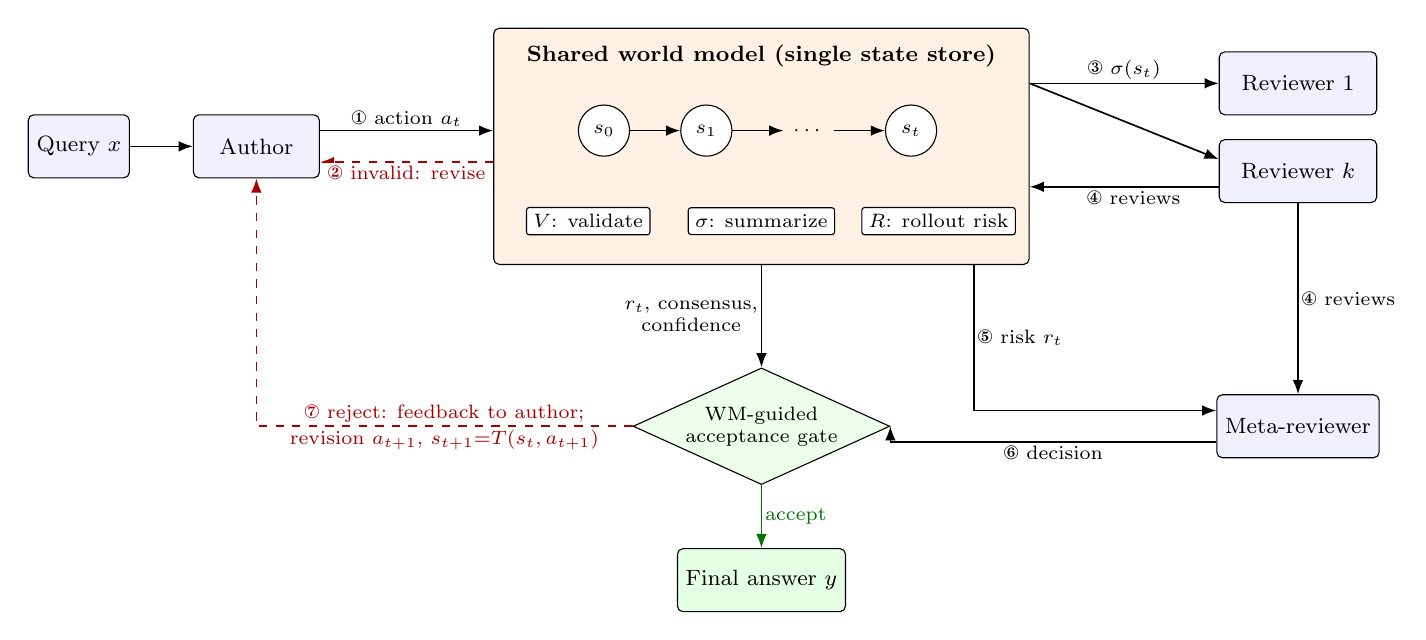
\begin{tikzpicture}[node distance=7mm and 12mm]
\node[agent] (q) {Query $x$};
\node[agent, right=8mm of q, minimum width=16mm] (a) {Author};
\node[wm, right=22mm of a, minimum width=68mm, minimum height=30mm] (w) {};
\node[ttl, anchor=north] at ([yshift=-1mm]w.north) {Shared world model (single state store)};
\node[st] (s0) at ([xshift=-20mm,yshift=2mm]w.center) {$s_0$};
\node[st] (s1) at ([xshift=-7mm,yshift=2mm]w.center) {$s_1$};
\node[font=\scriptsize] (sd) at ([xshift=6mm,yshift=2mm]w.center) {$\cdots$};
\node[st] (s2) at ([xshift=19mm,yshift=2mm]w.center) {$s_t$};
\draw[flow] (s0) -- (s1); \draw[flow] (s1) -- (sd); \draw[flow] (sd) -- (s2);
\node[op] (v) at ([xshift=-22mm,yshift=-9.5mm]w.center) {$V$: validate};
\node[op] (sg) at ([xshift=0mm,yshift=-9.5mm]w.center) {$\sigma$: summarize};
\node[op] (rr) at ([xshift=22.5mm,yshift=-9.5mm]w.center) {$R$: rollout risk};
\node[agent, right=24mm of w, yshift=8mm, minimum width=20mm] (r1) {Reviewer 1};
\node[agent, below=3mm of r1, minimum width=20mm] (r2) {Reviewer $k$};
\node[gate, below=13mm of w] (g) {WM-guided\\acceptance gate};
\node[agent, minimum width=20mm] (m) at (r2 |- g) {Meta-reviewer};
\node[agent, below=8mm of g, fill=green!10] (out) {Final answer $y$};

\draw[flow] (q) -- (a);
\draw[flow] ([yshift=2mm]a.east) -- node[lbl, above] {\ding{172} action $a_t$} ([yshift=2mm]a.east -| w.west);
\draw[fb] ([yshift=-2mm]a.east -| w.west) -- node[lbl, below] {\ding{173} invalid: revise} ([yshift=-2mm]a.east);
\draw[flow] ([yshift=8mm]w.east) -- node[lbl, above] {\ding{174} $\sigma(s_t)$} (r1.west);
\draw[flow] ([yshift=8mm]w.east) -- ([yshift=1.5mm]r2.west);
\draw[flow] ([yshift=-2mm]r2.west) -- node[lbl, below, pos=0.45] {\ding{175} reviews} ([yshift=-2mm]r2.west -| w.east);
\draw[flow] (r2) -- node[lbl, right] {\ding{175} reviews} (m);
\draw[flow] ([xshift=27mm]w.south) |- node[lbl, pos=0.25, right] {\ding{176} risk $r_t$} ([yshift=2mm]m.west);
\draw[flow] ([yshift=-2mm]m.west) -- node[lbl, below, pos=0.5] {\ding{177} decision} ([yshift=-2mm]m.west -| g.east) -- (g.east);
\draw[flow] (w.south) -- node[lbl, left] {$r_t$, consensus,\\confidence} (g.north);
\draw[flow, green!45!black] (g) -- node[lbl, right] {accept} (out);
\draw[fb] (g.west) -| node[lbl, pos=0.25, above] {\ding{178} reject: feedback to author;}  node[lbl, pos=0.25, below] {revision $a_{t+1}$, $s_{t+1}{=}T(s_t,a_{t+1})$} (a.south);
\end{tikzpicture}
}
    \caption{Centralized world-model coordination. All agents read from and write to one shared state store; the world model validates each action, distributes the state summary, computes the trajectory risk from the reviews, and gates acceptance.}
    \label{fig:centralized}
\end{figure*}

\subsubsection{Peer-to-peer coordination}
In the peer architecture (Fig.~\ref{fig:peer}) there is no shared state store. Every agent owns a local world-model instance.
The author commits and validates its candidates in its local instance and sends the resulting summary to the reviewers as part of its message; each reviewer and the meta-reviewer mirror the received information into their own local instances.
The meta-reviewer's local world model has no access to a shared review record and therefore computes only a local risk (Eq.~\eqref{eq:risk} without the review-dependent terms, with base level 0.5), which is reported in the meta-reviewer prompt.
There is no global gate: a candidate is accepted as soon as the meta-reviewer decides ``right''.
Peer coordination is thus the lighter mechanism. It keeps explicit state tracking and validation on the author side but leaves the acceptance decision to the agents, whereas centralized coordination adds a conservative, state-level check that can overrule them.

\begin{figure*}[!t]
    \centering
    \resizebox{0.95\textwidth}{!}{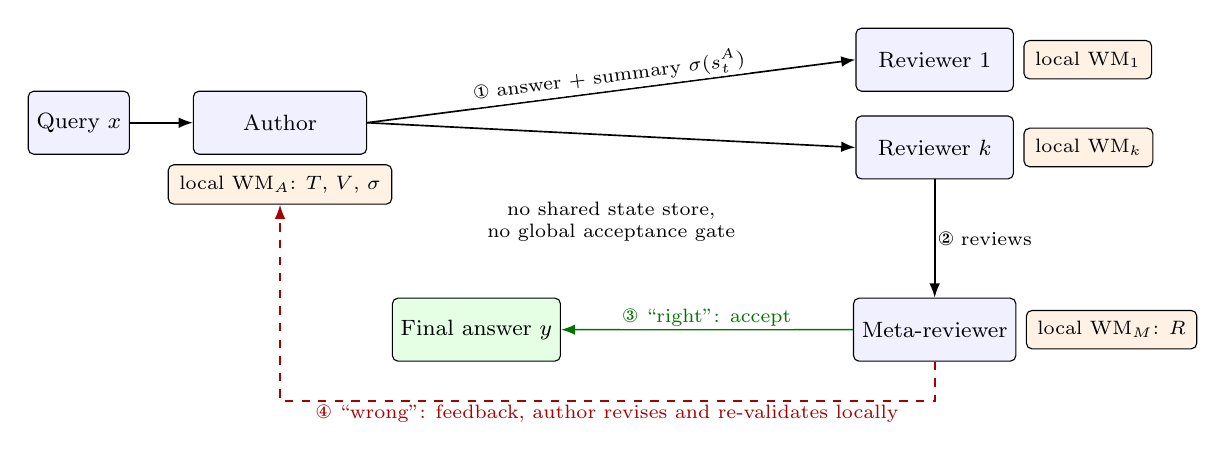
\begin{tikzpicture}[node distance=7mm and 12mm]
\node[agent] (q) {Query $x$};
\node[agent, right=8mm of q, minimum width=22mm] (a) {Author};
\node[wm, below=1.2mm of a, minimum width=22mm, font=\scriptsize] (wa) {local WM$_A$: $T$, $V$, $\sigma$};
\node[agent, right=62mm of a, yshift=8mm, minimum width=20mm] (r1) {Reviewer 1};
\node[wm, right=1.2mm of r1, font=\scriptsize] (w1) {local WM$_1$};
\node[agent, below=3mm of r1, minimum width=20mm] (r2) {Reviewer $k$};
\node[wm, right=1.2mm of r2, font=\scriptsize] (w2) {local WM$_k$};
\node[agent, below=15mm of r2, minimum width=20mm] (m) {Meta-reviewer};
\node[wm, right=1.2mm of m, font=\scriptsize] (wmm) {local WM$_M$: $R$};
\node[agent, fill=green!10] (out) at ($(a |- m)!0.3!(m)$) {Final answer $y$};
\node[font=\scriptsize, align=center, text width=44mm] at ($(a.east)!0.5!(r2.west)+(0,-11mm)$) {no shared state store,\\no global acceptance gate};

\draw[flow] (q) -- (a);
\draw[flow] (a.east) -- node[lbl, above, sloped] {\ding{172} answer + summary $\sigma(s^{A}_t)$} (r1.west);
\draw[flow] (a.east) -- (r2.west);
\draw[flow] (r2) -- node[lbl, right] {\ding{173} reviews} (m);
\draw[flow, green!45!black] (m.west) -- node[lbl, above] {\ding{174} ``right'': accept} (out.east);
\draw[fb] (m.south) -- ++(0,-5mm) -| node[lbl, pos=0.25, below] {\ding{175} ``wrong'': feedback, author revises and re-validates locally} (wa.south);
\end{tikzpicture}
}
    \caption{Peer-to-peer world-model coordination. Each agent keeps a local world-model replica; state summaries travel inside messages, and acceptance follows the meta-reviewer's decision.}
    \label{fig:peer}
\end{figure*}

\subsection{World-Model--Guided Acceptance}
\label{sec:gate}

In centralized mode a candidate that the meta-reviewer judges ``right'' is accepted only if it also passes the following gate.
Let \(\kappa\) be the number of reviewers counted as agreeing with the candidate (a reviewer agrees if its review has positive polarity or its reliability exceeds 0.7).
The risk is first adjusted by lexical cues in the meta-review, \(r'_t = \mathrm{clip}_{[0,1]}(r_t + \Delta_{\mathrm{meta}})\), where \(\Delta_{\mathrm{meta}}\in[-0.15,+0.25]\) is positive when the meta-review mentions flaws or concerns and negative when it states that the answer is clearly correct.
The \emph{effective risk} combines the adjusted risk with reviewer reliability,
\begin{equation}
\tilde r_t = 0.7\, r'_t + 0.3\,(1-\bar c),
\end{equation}
and is compared with a length-aware threshold \(\theta = \theta_0 + \min(0.12,\ L/900)\), where \(L\) is the number of words in the candidate.
The candidate is accepted if either
\begin{align}
&\tilde r_t \le \theta \ \wedge\ \kappa \ge \kappa_{\min} \ \wedge\ \bar c > c_{\min}, \quad\text{or} \label{eq:gateA}\\
&\kappa = k \ \wedge\ \bar c > c_{\mathrm{full}} \ \wedge\ \tilde r_t \le r_{\mathrm{cap}}. \label{eq:gateB}
\end{align}
Otherwise the meta-review is returned to the author as feedback, the author revises, and the revision is committed as a new state.
Table~\ref{tab:hyper} lists the gate hyperparameters. They are defined per answer format rather than per dataset and were fixed before the experiments reported in this paper.

\begin{table}[!t]
\caption{Acceptance-gate hyperparameters (centralized mode)}
\label{tab:hyper}
\centering
\footnotesize
\setlength{\tabcolsep}{3pt}
\begin{tabular}{lccccc}
\toprule
Task family & $\theta_0$ & $\kappa_{\min}$ & $c_{\min}$ & $c_{\mathrm{full}}$ & $r_{\mathrm{cap}}$ \\
\midrule
\makecell[l]{GSM8K, SVAMP,\\GSM-Hard, StrategyQA} & 0.28 & 2 & 0.65 & 0.80 & 0.45 \\
CIAR & 0.35 & 1 & 0.60 & 0.75 & 0.50 \\
MMLU subsets & 0.38 & 1 & 0.58 & 0.72 & 0.52 \\
\bottomrule
\end{tabular}
\end{table}

\subsection{Overall Procedure}

Algorithm~\ref{alg:wm-agent} summarizes one run. The same procedure covers both architectures; they differ in where the state lives and in the acceptance test of line~\ref{line:accept}.

\begin{algorithm}[t]
\caption{World-Model--Guided Multi-Agent Reasoning}
\label{alg:wm-agent}
\begin{algorithmic}[1]
\REQUIRE Query \(x\), reviewers \(k\), maximum review rounds \(N\)
\ENSURE Final answer \(y\)
\STATE \(s \leftarrow T(\varnothing, \langle\textsc{init}, x\rangle)\)
\STATE Author drafts candidate \(c\); \(a \leftarrow \langle\textsc{draft}, c\rangle\); \(s \leftarrow T(s, a)\)
\IF{\(V(s,a)\) fails}
    \STATE Author re-submits \(c\) given the validator hint; \(s \leftarrow T(s, \langle\textsc{revalidated}, c\rangle)\)
\ENDIF
\FOR{\(n = 1,\ldots,N\)}
    \STATE Each reviewer evaluates \(c\) given \(\sigma(s)\) \(\rightarrow\) reviews \(\mathcal{F}\)
    \STATE \(r \leftarrow R(s, \mathcal{F})\) \COMMENT{trajectory risk, Eq.~\eqref{eq:risk}}
    \STATE Meta-reviewer decides \(d\in\{\text{right},\text{wrong}\}\) given \(c, \mathcal{F}, r\)
    \IF{\(d=\text{right}\) \AND \textsc{Accept}\((r,\mathcal{F})\)} \label{line:accept}
        \RETURN answer of \(c\)
    \ENDIF
    \IF{\(n<N\)}
        \STATE Author revises \(c\) given the meta-review; \(a \leftarrow \langle\textsc{revision}, c\rangle\); \(s \leftarrow T(s,a,n)\)
        \STATE Re-submit once if \(V(s,a)\) fails
    \ENDIF
\ENDFOR
\RETURN answer of the last candidate \(c\)
\end{algorithmic}
\vspace{2pt}
{\footnotesize \textsc{Accept} is Eqs.~\eqref{eq:gateA}--\eqref{eq:gateB} in centralized mode and always true in peer mode.}
\end{algorithm}

\subsection{Coordination Uncertainty Index}
\label{sec:cui}

To characterize when each architecture is preferable we define the \emph{Coordination Uncertainty Index} (CUI), a dataset-level statistic computed from the logs of the first review round.
It is inspired by information-theoretic notions of uncertainty~\cite{shannon1948mathematical} and aggregates four signals of how hard it is for the agents to agree on a stable shared state.
For a dataset \(D\) with \(N\) tasks:

\begin{itemize}
\item \textbf{Reviewer belief entropy.} Let \(p^{(i)}\) be the fraction of reviewers whose decision on task \(i\) is ``right''. Then
\(H_{\mathrm{rev}} = \tfrac1N\sum_i \big[-p^{(i)}\log p^{(i)} - (1-p^{(i)})\log(1-p^{(i)})\big]\).
\item \textbf{Confidence dispersion.} \(V_{\mathrm{conf}} = \tfrac1N\sum_i \mathrm{Var}(c^{(i)}_1,\ldots,c^{(i)}_k)\), the variance of the reviewers' reliability scores.
\item \textbf{Risk instability.} \(V_{\mathrm{risk}} = \tfrac1N\sum_i \mathrm{Var}(r^{(i)}_1,\ldots,r^{(i)}_{n_i})\), the variance of the trajectory risk (Eq.~\eqref{eq:risk}) over the \(n_i\) review rounds of task \(i\) (zero for single-round tasks).
\item \textbf{Answer entropy.} \(H_{\mathrm{ans}}\) is the mean Shannon entropy of the multiset of normalized final answers proposed for a task by the author, the reviewers, and the meta-reviewer.
\end{itemize}

Each component is min--max normalized over the pool of datasets under study (denoted by a hat), and the index is their unweighted mean:
\begin{equation}
\label{eq:cui}
U(D) = \tfrac14\big(\hat H_{\mathrm{rev}} + \hat V_{\mathrm{conf}} + \hat V_{\mathrm{risk}} + \hat H_{\mathrm{ans}}\big).
\end{equation}
We use equal weights to avoid fitting additional free parameters on a small number of datasets.
Because of the normalization, \(U(D)\) is a \emph{relative} index: it ranks the datasets of a pool by coordination uncertainty, and a threshold \(\tau\) is meaningful only with respect to that pool.
Unless stated otherwise, the CUI is computed from peer-mode logs, which are the cheapest to obtain.

\section{Experimental Setup}
\label{sec:setup}

\subsection{Backbones and Inference Configuration}
\label{sec:llm}

All agents in a run share one backbone LLM. To test whether the findings depend on the backbone we use four OpenAI models that differ in capability: \texttt{gpt-3.5-turbo} (snapshot \texttt{gpt-3.5-turbo-0125}), \texttt{gpt-4o-mini} (snapshot \texttt{gpt-4o-mini-2024-07-18}), \texttt{gpt-4.1-nano} (snapshot \texttt{gpt-4.1-nano-2025-04-14}), and \texttt{gpt-4.1-mini} (snapshot \texttt{gpt-4.1-mini-2025-04-14}).
All models are accessed through the OpenAI Chat Completions API.
Every call uses temperature \(1.0\), the API defaults for nucleus sampling and output length, a fresh random seed, and \texttt{logprobs} enabled; the token log-probabilities are used only to compute the reviewer reliability score of Section~\ref{sec:wm}.
No system prompt, tool, or retrieval component is used.
All coordination strategies and all baselines use the same backbone, the same decoding configuration, and the same answer format within a comparison, so that differences in accuracy are attributable to the coordination strategy.
The reviewer-style configurations use one author, \(k=2\) reviewers, one meta-reviewer, and at most \(N=3\) review rounds.

\subsection{Benchmarks}

We evaluate on eight reasoning benchmarks (Table~\ref{tab:dataset_overview}):
\textbf{GSM8K}~\cite{cobbe2021gsm8k}, grade-school math word problems;
\textbf{SVAMP}~\cite{patel2021svamp}, arithmetic word problems with structural perturbations;
\textbf{GSM-Hard}~\cite{gao2023pal}, GSM8K problems with numbers replaced by large values;
\textbf{CIAR}~\cite{liang2024mad}, counter-intuitive arithmetic reasoning problems;
\textbf{StrategyQA}~\cite{geva2021strategyqa}, yes/no questions that require implicit multi-hop reasoning;
and three subsets of \textbf{MMLU}~\cite{hendrycks2021mmlu}: \emph{elementary mathematics}, \emph{moral scenarios}, and \emph{professional law}.
The first four benchmarks have numeric answers (scored correct within an absolute tolerance of \(0.01\)); the others are multiple-choice or binary and are scored by exact match of the selected option.

For each benchmark we fix one list of 50 question indices (all 48 questions for CIAR), sampled once, and evaluate \emph{every} method and \emph{every} backbone on exactly these questions, giving 398 questions per backbone.
The three reviewer-style configurations are run with all four backbones in two independent runs (1{,}592 paired questions, 3{,}184 runs per configuration in total), the external baselines once with \texttt{gpt-4.1-mini} and \texttt{gpt-4.1-nano}, and the ablations once with \texttt{gpt-4o-mini}, the backbone on which the centralized gate had the largest effect in the first run.
A disjoint set of 30 further questions per benchmark (210 in total; CIAR has no unused questions) is reserved as a development split for the exploratory variants of Sections~\ref{sec:pilot}--\ref{sec:combined}.

\begin{table}[!t]
\caption{Evaluation Benchmarks}
\label{tab:dataset_overview}
\centering
\footnotesize
\setlength{\tabcolsep}{3pt}
\begin{tabular}{llll}
\toprule
Benchmark & Domain & Answer & \#Q \\
\midrule
GSM8K & Math word problems & Numeric & 50 \\
SVAMP & Math word problems & Numeric & 50 \\
GSM-Hard & Math, large numbers & Numeric & 50 \\
MMLU-Elem. & Elementary mathematics & 4-way MC & 50 \\
CIAR & Counter-intuitive arithmetic & Numeric & 48 \\
StrategyQA & Implicit multi-hop QA & Binary & 50 \\
MMLU-Moral & Moral scenarios & 4-way MC & 50 \\
MMLU-Law & Professional law & 4-way MC & 50 \\
\bottomrule
\end{tabular}
\end{table}

\subsection{Compared Methods}

\paragraph{Reviewer-style configurations.}
\emph{Reviewer pipeline} is the message-based author--reviewer--meta-reviewer pipeline of MARS~\cite{wang2025mars} without any world model; it accepts a candidate when the meta-reviewer decides ``right''.
\emph{Ours (Peer)} and \emph{Ours (Centralized)} add the world model of Section~\ref{sec:method} in the two coordination architectures.
The three configurations share all prompts.

\paragraph{External baselines.}
We re-implement six methods in the same evaluation pipeline, with the same backbone and answer format:
\emph{CoT}, a single chain-of-thought call~\cite{wei2022chain};
\emph{Self-Consistency} with five samples and majority voting~\cite{wang2023selfconsistency};
\emph{Self-Reflection}, one answer followed by one self-critique and revision~\cite{madaan2023selfrefine,shinn2023reflexion};
\emph{Multi-Agent Debate} with three agents and two rounds~\cite{du2024improving};
\emph{MAD} with an affirmative debater, a negative debater, and a judge that may stop the debate, for at most three rounds~\cite{liang2024mad};
and \emph{ReConcile} with three agents, at most three discussion rounds, and confidence-weighted voting~\cite{chen2024reconcile}.
ReConcile was proposed for a mixture of different LLMs; to keep the backbone fixed we use its single-backbone variant and omit its ``convincing samples'' component.
We do not include AgentVerse or GPTSwarm as baselines: the former recruits task-specific expert roles and the latter optimizes a graph on a training split, so neither can be reproduced faithfully in a setting with a fixed role set and no training data.

\paragraph{Ablations.}
Starting from the centralized configuration we remove one world-model component at a time:
(i) \emph{w/o shared state summary}: reviewers do not receive \(\sigma(s_t)\);
(ii) \emph{w/o transition validation}: \(V\) is skipped;
(iii) \emph{w/o trajectory risk}: \(R\) is not computed, so the risk is neither shown to the meta-reviewer nor used in the gate (the consensus and reliability conditions remain);
(iv) \emph{w/o WM-guided acceptance}: the gate of Section~\ref{sec:gate} is removed and acceptance follows the meta-reviewer, while state, validation, and risk reporting remain.

\subsection{Metrics and Statistical Analysis}

We report accuracy, the average number of tokens (prompt plus completion) per question, the average number of LLM calls per question, and the average wall-clock time per question.
Because individual benchmarks contain at most 50 questions, per-benchmark differences below roughly 15 percentage points cannot be resolved, and we base our conclusions on comparisons pooled over benchmarks. We accompany accuracy differences with paired tests: for two methods evaluated on the same questions we compute the per-question difference in correctness, a 95\% bootstrap confidence interval of its mean, and a two-sided paired sign-flip permutation test (20{,}000 permutations).
We do not correct for multiple comparisons and therefore treat per-dataset \(p\)-values as descriptive.
Every number in the tables and figures of this paper is generated by a single analysis script from the per-question run logs.


\section{Results}
\label{sec:results}

\subsection{RQ1: Accuracy and Cost of World-Model--Guided Coordination}
\label{sec:main_results}

\begin{table*}[!t]
\caption{Accuracy (\%) of the Three Reviewer-Style Configurations on Identical Questions (50 per Benchmark, 48 for CIAR). Rev.: Message-Based Reviewer Pipeline. Bold: best per backbone and benchmark. The last row is the macro-average over benchmarks.}
\label{tab:main_results}
\centering
\small
\setlength{\tabcolsep}{3.5pt}
\begin{tabular}{l ccc ccc ccc ccc}
\toprule
 & \multicolumn{3}{c}{GPT-3.5-Turbo} & \multicolumn{3}{c}{GPT-4o-mini} & \multicolumn{3}{c}{GPT-4.1-nano} & \multicolumn{3}{c}{GPT-4.1-mini} \\
\cmidrule(lr){2-4}\cmidrule(lr){5-7}\cmidrule(lr){8-10}\cmidrule(lr){11-13}
Benchmark & Rev. & Peer & Centr. & Rev. & Peer & Centr. & Rev. & Peer & Centr. & Rev. & Peer & Centr. \\
\midrule
\tabinput{tables/main_results.tex}
\bottomrule
\end{tabular}
\end{table*}

\begin{table*}[!t]
\caption{Pooled Paired Comparisons Over All Questions. Differences Are in Accuracy Points With 95\% Bootstrap Confidence Intervals; $p$: Two-Sided Paired Permutation Test.}
\label{tab:pooled}
\centering
\small
\setlength{\tabcolsep}{4pt}
\begin{tabular}{l c ccc cc cc cc}
\toprule
 & & \multicolumn{3}{c}{Accuracy (\%)} & \multicolumn{2}{c}{Peer $-$ Reviewer} & \multicolumn{2}{c}{Centr. $-$ Reviewer} & \multicolumn{2}{c}{Centr. $-$ Peer} \\
\cmidrule(lr){3-5}\cmidrule(lr){6-7}\cmidrule(lr){8-9}\cmidrule(lr){10-11}
Backbone & $n$ & Reviewer & Peer & Centr. & $\Delta$ [95\% CI] & $p$ & $\Delta$ [95\% CI] & $p$ & $\Delta$ [95\% CI] & $p$ \\
\midrule
\tabinput{tables/pooled.tex}
\bottomrule
\end{tabular}
\end{table*}

Table~\ref{tab:main_results} reports per-benchmark accuracy and Table~\ref{tab:pooled} the pooled paired comparisons.

\paragraph{Peer-to-peer coordination does not differ from the message-based pipeline.}
The pooled difference between the peer configuration and the reviewer pipeline is \(-0.5\), \(+1.5\), \(+2.0\), and \(0.0\) points on the four backbones and \(+0.8\) points overall (\(p=0.43\)); none of the per-backbone differences approaches significance.
This is consistent with the design of the peer mode: it adds explicit state tracking and validation on the author side and a state summary in the reviewer prompts, but it leaves the acceptance rule of the pipeline unchanged.

\paragraph{Centralized coordination helps on one backbone.}
With GPT-4o-mini the centralized configuration is at least as accurate as the reviewer pipeline on all eight benchmarks and \(4.0\) points better overall (95\% CI \([+0.5,+7.3]\), \(p=0.032\)).
With GPT-4.1-nano the difference is \(+3.5\) points (\(p=0.071\)), with GPT-3.5-Turbo it is \(-0.8\) points (\(p=0.83\)), and with GPT-4.1-mini it is \(-2.3\) points (\(p=0.14\)).
Pooled over the four backbones the gain is \(+1.1\) points and not significant (\(p=0.24\)).
Section~\ref{sec:gate_results} shows that part of these between-run differences is sampling variation in the authors' first drafts, and gives a cleaner within-run estimate.

\paragraph{No benchmark-level regime.}
None of the 32 backbone--benchmark combinations shows a significant difference between the peer and the centralized configuration (smallest \(p=0.059\), uncorrected).
In particular, the data do not support a pattern in which centralized coordination wins on structured arithmetic benchmarks and peer coordination wins on ambiguous ones: for almost every benchmark the sign of the peer--centralized gap changes from one backbone to the next (for example, on GSM8K it is \(+6\), \(-2\), \(-6\), and \(+2\) points for the four backbones).

\paragraph{Cost.}
Table~\ref{tab:efficiency} shows that the peer configuration costs about as much as the reviewer pipeline, whereas with GPT-4o-mini the centralized configuration uses \(3.8\times\) the tokens and roughly twice the LLM calls, because its gate triggers additional review rounds (the ratio is \(1.6\times\) for GPT-3.5-Turbo, \(3.7\times\) for GPT-4.1-nano, and \(4.2\times\) for GPT-4.1-mini; Table~\ref{tab:gate}).
The overhead grows with task difficulty: on MMLU-Law the centralized configuration consumes more than five times the tokens of the reviewer pipeline.

\begin{table}[!t]
\caption{Cost per Question With GPT-4o-mini: Tokens, LLM Calls, and Wall-Clock Time (s, Measured Under Concurrent Execution). R: Reviewer Pipeline, P: Peer, C: Centralized.}
\label{tab:efficiency}
\centering
\footnotesize
\setlength{\tabcolsep}{2.5pt}
\begin{tabular}{l rrr rrr rrr}
\toprule
 & \multicolumn{3}{c}{Tokens} & \multicolumn{3}{c}{Calls} & \multicolumn{3}{c}{Time} \\
\cmidrule(lr){2-4}\cmidrule(lr){5-7}\cmidrule(lr){8-10}
Benchmark & R & P & C & R & P & C & R & P & C \\
\midrule
\tabinput{tables/efficiency.tex}
\bottomrule
\end{tabular}
\end{table}

\subsection{RQ2: What the Review Process and the Gate Actually Do}
\label{sec:gate_results}

Because the author's first draft is logged in every run, we can measure the effect of each configuration within a run, as the change from draft accuracy to final accuracy. This removes the variation between independently sampled drafts that affects Table~\ref{tab:pooled}.
Table~\ref{tab:gate} reports this quantity together with statistics of the first-round acceptance decision.

\begin{table*}[!t]
\caption{Within-Run Effect of Each Configuration (398 Questions per Row). Draft/Final: Accuracy (\%) of the Author's First Draft and of the Returned Answer. W$\to$R / R$\to$W: Share of Runs (\%) Whose Answer Changes From Wrong to Right / Right to Wrong. Pass: Share (\%) of Correct and of Incorrect Drafts Accepted in the First Round. Repaired: Share (\%) of Incorrect Drafts Not Accepted in the First Round That End Correct (Count of Such Drafts in Parentheses).}
\label{tab:gate}
\centering
\small
\setlength{\tabcolsep}{4.5pt}
\begin{tabular}{ll ccc cc cc c cc}
\toprule
 & & \multicolumn{3}{c}{Accuracy} & \multicolumn{2}{c}{Flips} & \multicolumn{2}{c}{Pass in round 1} & & & \\
\cmidrule(lr){3-5}\cmidrule(lr){6-7}\cmidrule(lr){8-9}
Backbone & Configuration & Draft & Final & Net & W$\to$R & R$\to$W & Correct & Incorrect & Repaired & Rounds & Tokens \\
\midrule
\tabinput{tables/gate.tex}
\bottomrule
\end{tabular}
\end{table*}

\paragraph{Without a gate, review is close to a rubber stamp.}
In the reviewer pipeline and in the peer configuration, 81--99\% of incorrect drafts are accepted in the first round, because the meta-reviewer judges them ``right''.
The average number of review rounds is between 1.00 and 1.16, and the net change from draft to final accuracy is at most \(+2.3\) points; it is nominally significant in one of the eight cases (peer with GPT-4.1-nano, \(p=0.04\), uncorrected).
With GPT-4.1-mini the reviewer pipeline changes the outcome of one question out of 398.
The four-agent pipeline therefore returns, in the large majority of cases, the answer that a single call would have produced.

\paragraph{The gate intervenes, but with little discrimination.}
With the three more recent backbones the centralized gate reduces the first-round acceptance of incorrect drafts to 19--27\%.
It does so, however, mainly by being strict rather than by being selective: it also withholds acceptance from 56--60\% of \emph{correct} drafts.
With GPT-3.5-Turbo the same gate, with the same thresholds, is lenient instead: it passes 82\% of correct and 64\% of incorrect drafts. The behaviour of a gate built on reviewer confidence and review wording therefore does not transfer across backbones without recalibration.
The gate thus roughly doubles the number of review rounds for correct and incorrect drafts alike, which explains the cost in Table~\ref{tab:efficiency}.

\paragraph{Blocked errors are rarely repaired.}
What happens after a block determines the benefit.
With GPT-4o-mini, 34\% of the blocked incorrect drafts end with a correct answer, giving a net within-run gain of \(+4.3\) points (\(p=0.010\), paired test of final against draft).
With GPT-3.5-Turbo and GPT-4.1-nano the repair rates are 18\% and 12\% and the net gains \(+1.3\) points each (not significant); with GPT-4.1-mini the repair rate is 5\%, and the net gain is zero: the author is asked to revise 61 incorrect drafts and corrects three of them, while three initially correct answers are lost.
The strongest backbone is thus the one that benefits least: its reviewers and meta-reviewer agree with the draft almost unconditionally, and its author rarely departs from its first answer when asked to revise.

\paragraph{Reading Table~\ref{tab:pooled} in this light.}
The within-run estimates (\(+1.3\), \(+4.3\), \(+1.3\), and \(0.0\) points for the four backbones) are the appropriate measure of what the gate contributes.
The between-run difference of \(-2.3\) points for GPT-4.1-mini in Table~\ref{tab:pooled} mostly reflects that the drafts sampled in the centralized runs happened to be two points less accurate than those sampled in the reviewer-pipeline runs (78.9\% versus 80.9\%), not a harmful effect of the gate.

\IfFileExists{sec_ablation.tex}{\subsection{Ablation of World-Model Components}
\label{sec:ablation}

To see which component of the centralized configuration is responsible for its behaviour we remove them one at a time with GPT-4o-mini (Table~\ref{tab:ablation}).
Each variant is run once on the same 398 questions; for comparability the table shows the \emph{first} run of the two reference configurations, which were run in the same batch.

\begin{table*}[!t]
\caption{Ablation with GPT-4o-mini (398 questions per row, single run). Columns as in Table~\ref{tab:gate}; $\Delta$ Full: paired difference in final accuracy to the full centralized configuration in the same run (points, $p$ of the paired permutation test in parentheses).}
\label{tab:ablation}
\footnotesize
\setlength{\tabcolsep}{3pt}
\resizebox{\linewidth}{!}{\begin{tabular}{l ccc cc cc c cc c}
\toprule
 & \multicolumn{3}{c}{Accuracy} & \multicolumn{2}{c}{Flips} & \multicolumn{2}{c}{Pass in round 1} & & & & \\
\cmidrule(lr){2-4}\cmidrule(lr){5-6}\cmidrule(lr){7-8}
Configuration & Draft & Final & Net & W$\to$R & R$\to$W & Correct & Incorrect & Repaired & Rounds & Tokens & $\Delta$ Full \\
\midrule
\tabinput{tables/ablation.tex}
\bottomrule
\end{tabular}}
\end{table*}

\paragraph{Accuracy differences are within run-to-run variation.}
The run of the full configuration that serves as reference is the one that gained \(+4.3\) points over its drafts; its second run gained \(-0.8\) (Section~\ref{sec:main_results}).
The four variants gain \(+1.3\) to \(+2.3\) points, i.e., about as much as the ungated pipeline and as the full configuration in its second run.
We therefore do not read the \(\Delta\)~Full column as component contributions: the one nominally significant entry (without the state summary, \(-3.8\) points, \(p=0.02\)) is of the size of the difference between the two runs of the unmodified system.
Running each variant repeatedly would be required to resolve accuracy effects of this size, and the main-result experiment suggests there are none to resolve.

\paragraph{Behaviour and cost are stable and informative.}
The behavioural columns do not depend on the sampling of drafts in the same way, and they tell a consistent story.
Removing the state summary, validation, or the risk estimate leaves the gate's behaviour unchanged: 39--43\% of correct and 14--19\% of incorrect drafts pass, rounds stay at 2.3, and tokens at 15--16k.
Transition validation in particular changes nothing, which is expected since its lexicon-based checks fire rarely.
The variant \emph{without the acceptance gate}, in which the world model still validates, summarizes, and reports the risk to the meta-reviewer but acceptance follows the meta-reviewer's verdict, is the informative one: reporting the risk lowers the first-round acceptance of incorrect drafts from 85\% to 78\% while 97\% of correct drafts still pass, at 1.08 rounds and \(4.8\)k tokens---a third of the cost of gating.
Whatever behavioural effect the full gate has on the collective's willingness to reconsider is thus obtained largely by making the risk visible, and the forced additional rounds (which cost roughly 11k tokens per question) do not turn that reconsideration into measurable accuracy.
}{}

\subsection{RQ3: Does Coordination Uncertainty Predict the Preferable Mode?}
\label{sec:cui_results}

We now test the hypothesis of Eq.~\eqref{eq:policy}: that datasets with low CUI favor centralized coordination and datasets with high CUI favor peer coordination.
Table~\ref{tab:cui} lists, for each backbone, the CUI of every benchmark (computed from that backbone's peer-mode logs) and the accuracy gap \(\Delta = \mathrm{Acc}_{\mathrm{peer}} - \mathrm{Acc}_{\mathrm{centralized}}\); Fig.~\ref{fig:cui_regime} plots them.

\begin{table}[!t]
\caption{CUI and Peer$-$Centralized Accuracy Gap $\Delta$ (Points) per Benchmark, and Their Correlation Across the Eight Benchmarks}
\label{tab:cui}
\centering
\footnotesize
\setlength{\tabcolsep}{2.5pt}
\begin{tabular}{l cc cc cc cc}
\toprule
 & \multicolumn{2}{c}{3.5-Turbo} & \multicolumn{2}{c}{4o-mini} & \multicolumn{2}{c}{4.1-nano} & \multicolumn{2}{c}{4.1-mini} \\
\cmidrule(lr){2-3}\cmidrule(lr){4-5}\cmidrule(lr){6-7}\cmidrule(lr){8-9}
Benchmark & CUI & $\Delta$ & CUI & $\Delta$ & CUI & $\Delta$ & CUI & $\Delta$ \\
\midrule
\tabinput{tables/cui_compact.tex}
\bottomrule
\end{tabular}
\end{table}

\begin{figure*}[!t]
\centering
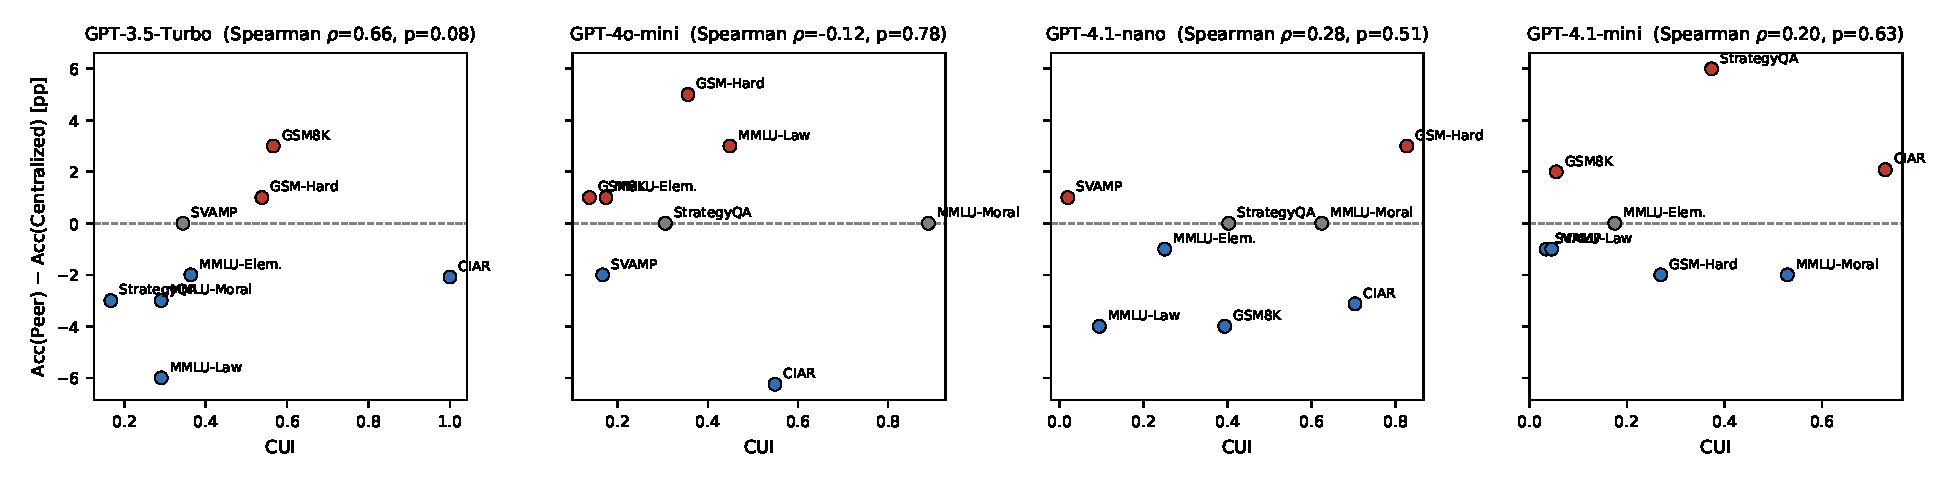
\includegraphics[width=0.95\textwidth]{figures/cui_scatter.pdf}
\caption{CUI versus the peer$-$centralized accuracy gap. Each point is a benchmark. The sign and strength of the association differ across backbones.}
\label{fig:cui_regime}
\end{figure*}

\paragraph{The association is not consistent across backbones.}
With GPT-4.1-mini the correlation has the hypothesized sign (Pearson \(r=+0.78\), Spearman \(\rho=+0.74\), \(p=0.036\)); with GPT-4.1-nano it is weaker and not significant (\(\rho=+0.42\), \(p=0.30\)); with GPT-3.5-Turbo there is no association (\(\rho=+0.04\), \(p=0.93\)); and with GPT-4o-mini it has the \emph{opposite} sign (\(r=-0.76\), \(\rho=-0.58\)): there, centralized coordination has its largest advantage on the benchmarks with the highest CUI (MMLU-Moral, CIAR).
With eight benchmarks per backbone and accuracy gaps that are individually not significant, each of these correlations is fragile, and together they give no support for a backbone-independent regime rule.
The result is also sensitive to the logs from which the CUI is computed: when it is computed from reviewer-pipeline logs instead of peer-mode logs, the correlation for GPT-4.1-mini drops to \(\rho=+0.34\) (\(p=0.40\)).

\paragraph{Threshold sensitivity.}
Fig.~\ref{fig:threshold} shows the macro-averaged accuracy of the policy of Eq.~\eqref{eq:policy} as the threshold \(\tau\) is varied over its whole range, with the two fixed policies and the per-benchmark oracle for reference.
For GPT-4o-mini the best threshold is \(\tau\ge 0.9\), i.e., always centralized; for GPT-4.1-mini it is \(\tau\le 0.04\), i.e., always peer; in both cases no threshold improves on the better fixed mode.
For GPT-4.1-nano thresholds in \([0.42, 0.70]\) exceed the better fixed mode by \(0.8\) points in-sample, and for GPT-3.5-Turbo thresholds in \([0.30, 0.34]\) exceed it by \(2.0\) points.
The per-benchmark oracle itself is between \(0.0\) and \(3.0\) points above the better fixed mode, so there is little to gain from mode selection on these benchmarks even with perfect information.
No single value of \(\tau\) is good for all four backbones: \(\tau=0.3\) is the best choice for GPT-3.5-Turbo but costs \(2.2\) points relative to the better fixed mode for GPT-4o-mini.

\begin{figure*}[!t]
\centering
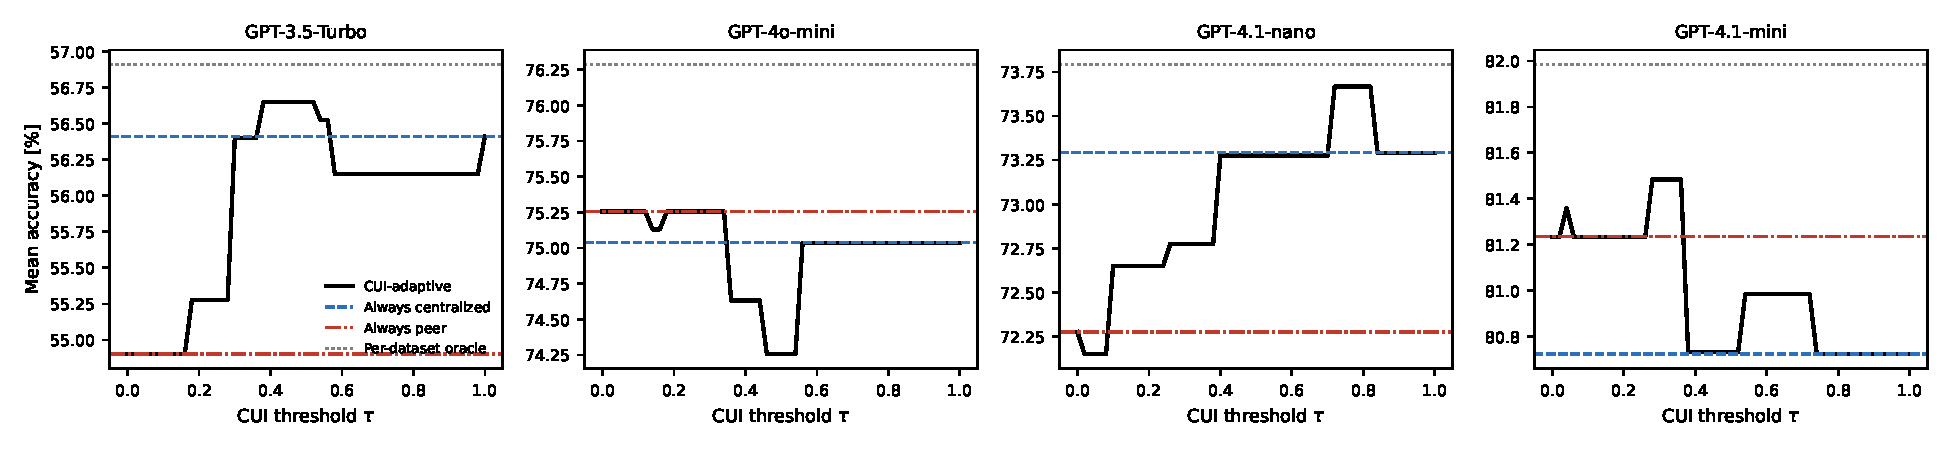
\includegraphics[width=0.95\textwidth]{figures/threshold_sensitivity.pdf}
\caption{Sensitivity of the CUI-adaptive policy to the threshold $\tau$ (macro-averaged accuracy over the eight benchmarks).}
\label{fig:threshold}
\end{figure*}

\paragraph{Held-out evaluation.}
To rule out that the in-sample analysis is too pessimistic or too optimistic, we also evaluate the rule out of sample: the CUI of a benchmark is computed on one half of its questions, \(\tau\) is chosen on the other seven benchmarks, and the selected mode is scored on the held-out half.
The adaptive policy reaches 57.1\%, 76.3\%, 73.8\%, and 83.4\% on the four backbones, against 56.1\%, 76.3\%, 74.3\%, and 83.4\% for the better fixed mode: it is one point better on one backbone, half a point worse on another, and identical on two.

\paragraph{Finer granularity.}
We repeated the analysis at the level of individual tasks and of batches of 5, 10, and 20 tasks (Table~\ref{tab:fine}).
A logistic model that predicts from the CUI whether peer coordination outperforms centralized coordination has a cross-validated AUC (folds grouped by benchmark) between 0.06 and 0.88, with no consistent trend in batch size or backbone, and its cross-validated accuracy never exceeds the majority-class rate by a meaningful margin.

\begin{table}[!t]
\caption{Predicting ``Peer Better Than Centralized'' From the CUI at Task and Batch Level. $R^2$: Linear Fit of the Accuracy Gap. AUC: In-Sample. CV: Cross-Validation Grouped by Benchmark.}
\label{tab:fine}
\centering
\footnotesize
\setlength{\tabcolsep}{3pt}
\begin{tabular}{llccccc}
\toprule
Backbone & Batch & $n$ & $R^2$ & AUC & CV Acc. & CV AUC \\
\midrule
\tabinput{tables/fine_grained.tex}
\bottomrule
\end{tabular}
\end{table}

In summary, the answer to RQ3 is negative: on the benchmarks and backbones studied here, the CUI is a descriptive statistic of reviewer disagreement, not a usable selector of the coordination mode.

\subsection{RQ4: Comparison With External Baselines}
\label{sec:baseline_results}

\begin{table*}[!t]
\caption{Accuracy (\%) of External Baselines and Reviewer-Style Configurations Under Identical Conditions. Tokens: Average per Question. Bold: Best per Column and Backbone.}
\label{tab:baselines}
\centering
\footnotesize
\setlength{\tabcolsep}{3.5pt}
\begin{tabular}{l cccccccc c r}
\toprule
Method & GSM8K & SVAMP & GSM-Hard & MMLU-El. & CIAR & StrategyQA & MMLU-Mor. & MMLU-Law & Avg. & Tokens \\
\midrule
\multicolumn{11}{l}{\emph{GPT-4.1-mini}} \\
\tabinput{tables/baselines_gpt-4.1-mini.tex}
\midrule
\multicolumn{11}{l}{\emph{GPT-4.1-nano}} \\
\tabinput{tables/baselines_gpt-4.1-nano.tex}
\bottomrule
\end{tabular}
\end{table*}

Table~\ref{tab:baselines} compares the reviewer-style configurations with six external baselines on two backbones.
Three observations stand out.
First, the spread among methods is small. Apart from MAD, which is clearly weaker, all methods lie within 3.5 points of each other in macro-averaged accuracy on GPT-4.1-mini (78.8--82.3\%) and within 3.5 points on GPT-4.1-nano (69.8--73.3\%); with 398 questions per cell, most of these differences are within sampling error.
Second, a single chain-of-thought call is a strong baseline: the best multi-agent method exceeds it by 1.2 points on GPT-4.1-mini (Multi-Agent Debate) and by 2.0 points on GPT-4.1-nano (centralized), while using 10 to 40 times as many tokens.
Third, the centralized configuration has no stable rank: it has the highest average on GPT-4.1-nano and the second lowest on GPT-4.1-mini, and it is the most expensive method on both.
We therefore do not claim that world-model--guided coordination outperforms existing multi-agent reasoning methods.

\IfFileExists{sec_pilot.tex}{\subsection{Exploratory Variant: An Answer-Agreement Gate}
\label{sec:pilot}

The diagnosis of Section~\ref{sec:gate_results} suggests two changes: base the acceptance decision on evidence that is more directly tied to correctness than the reviewers' stated opinions, and give the author more to work with when a draft is sent back.
We tested one simple instantiation on a development split that is disjoint from all questions used above (30 further questions from each benchmark except CIAR, which has no unused questions; 210 questions; GPT-4.1-mini, the backbone on which the centralized gate was least effective).
In this variant there is no meta-reviewer and no risk function. Each reviewer still solves the problem itself, and a draft is accepted if and only if the final answers of all reviewers equal the author's answer. On disagreement the author receives the reviewers' complete solutions and is asked to locate the step at which they diverge before answering again; if no agreement is reached after three rounds, the majority answer is returned.
This experiment is exploratory: it was designed after the main results were known and was run once.

\begin{table}[!t]
\caption{Exploratory Comparison on the Development Split (210 Questions, GPT-4.1-mini). Columns as in Table~\ref{tab:gate}.}
\label{tab:pilot}
\centering
\scriptsize
\setlength{\tabcolsep}{2.5pt}
\resizebox{\linewidth}{!}{\begin{tabular}{l ccc cc c r}
\toprule
 & \multicolumn{3}{c}{Accuracy} & \multicolumn{2}{c}{Pass in round 1} & & \\
\cmidrule(lr){2-4}\cmidrule(lr){5-6}
Configuration & Draft & Final & Net & Correct & Incorr. & Repaired & Tokens \\
\midrule
Reviewer pipe. & 80.5 & 81.4 & $+1.0$ & 100 & 95 & 100 (2) & 3.4k \\
Centralized & 83.8 & 86.2 & $+2.4$ & 44 & 21 & 19 (27) & 14.6k \\
Agreement gate & 83.3 & 85.2 & $+1.9$ & 98 & 80 & 71 (7) & 2.3k \\
\bottomrule
\end{tabular}}
\end{table}

Table~\ref{tab:pilot} shows that the agreement gate fixes one of the two weaknesses and exposes the other.
It is far more selective than the risk-based gate: it accepts 98\% of correct drafts in the first round (against 44\%), so it adds almost no rounds, and it uses 0.66 times the tokens of the reviewer pipeline and 0.15 times those of the centralized configuration.
When it does block an incorrect draft, the author repairs it in five of seven cases, compared with five of 27 for the centralized configuration, which indicates that showing the author concrete alternative solutions is more effective than returning a meta-review.
Its within-run gain (\(+1.9\) points) is comparable to that of the centralized configuration (\(+2.4\)); neither is significant on 210 questions (\(p=0.22\) and \(p=0.06\)).
All three configurations were run once on this split, so, as Table~\ref{tab:repcons} shows for the main split, accuracy differences of this size are within run-to-run variation; the behavioural columns (acceptance and repair rates, rounds, tokens) are the robust content of the table.

The remaining weakness is recall: 80\% of incorrect drafts still pass, because in 28 of 35 cases both reviewers arrive at the same incorrect answer as the author.
The errors of agents that share a backbone are strongly correlated, and in our pipeline the reviewer prompt also contains the author's draft, which may anchor the reviewers despite the instruction to solve the problem first.
An acceptance test based on agreement can therefore only be as good as the independence of the solvers.
Reviewers that never see the draft, and solvers drawn from different backbones as in ReConcile~\cite{chen2024reconcile}, are the obvious next steps; we leave them to future work and do not draw conclusions about accuracy from this exploratory comparison.
}{}

\section{Discussion}
\label{sec:discussion}

\paragraph{What an explicit state buys, and what it does not.}
Our results separate two things that are often conflated. Representing the reasoning state explicitly---storing candidates, validating transitions, showing reviewers a state summary---has no measurable effect by itself: the peer configuration, which does all of this, behaves like the message-based pipeline. What changes outcomes is an independent signal that reaches the deciding agent and, at a price, a gate that can overrule it. Inside the gated configuration the state summary does matter (Table~\ref{tab:ablation}): it raises the share of sent-back drafts that the author repairs. The useful part of the ``world model'' in our framework is therefore its role as an independent arbiter and as a carrier of evidence into the revision loop, not its role as a store.

\paragraph{Why the arbiter is weak.}
The trajectory risk of Eq.~\eqref{eq:risk} is built from signals that are only loosely related to correctness: lexical polarity of the reviews and the reviewers' token-level confidence. Since reviewers approve most drafts, right or wrong, these signals separate correct from incorrect drafts poorly (40--44\% versus 19--27\% first-round acceptance on the three more recent backbones), and the gate acts largely as a mechanism that forces extra rounds. Extra rounds help only if the author is able to revise, which Table~\ref{tab:gate} shows to be strongly backbone-dependent.

\paragraph{Agreement bias.}
The most robust observation in this study is that LLM reviewers and meta-reviewers agree with the answer in front of them, even though each reviewer is instructed to solve the problem independently before looking at the draft. This holds for all four backbones and is strongest for the most capable one. It suggests that critique-based multi-agent pipelines of this kind should be evaluated not only by final accuracy but by how often they change an answer and in which direction; the statistics of Table~\ref{tab:gate} are cheap to collect and considerably more informative than accuracy alone.

\paragraph{Limitations.}
(i) Each benchmark contributes at most 50 questions, so only pooled effects of a few points can be detected; per-benchmark conclusions should not be drawn from Table~\ref{tab:main_results}.
(ii) Each configuration was run once at temperature 1.0; repeated runs would reduce the draft-sampling variation that affects between-run comparisons.
(iii) All backbones are small models from one provider. The trend across them (less benefit for the stronger model) may or may not extend to frontier models.
(iv) The world model is rule-based, and its constants and the gate thresholds of Table~\ref{tab:hyper} were chosen by hand; a learned risk estimator could behave differently.
(v) Answers are extracted with the scoring script of the underlying pipeline~\cite{wang2025mars}, which can mis-parse numbers written with thousands separators; this affects all methods alike but lowers absolute accuracy on GSM-Hard.
(vi) The benchmarks are abstract reasoning tasks. We make no claim about embodied or cyber-physical settings, where a world model would have to represent physical dynamics; whether state-level gating is more valuable there is an open question.

\section{Conclusion}

We set out to test whether world-model principles---explicit state, validated transitions, and trajectory-level evaluation---improve coordination in multi-agent LLM reasoning.
In a controlled comparison on identical questions, explicit state tracking alone made no measurable difference, and a centralized state-level acceptance gate produced a significant gain on one of four backbones, at up to four times the token cost.
A coordination-uncertainty index did not predict which coordination mode is preferable.
The underlying reason is visible in the run logs: reviewer agents approve most incorrect answers, the gate cannot tell correct from incorrect drafts well, and authors seldom repair an answer that has been sent back.
These observations, together with the ablation and the exploratory variant, point away from richer state representations and toward two concrete targets for future work: acceptance signals that are grounded in independently derived answers rather than in the reviewers' stated opinions, and revision procedures that give the author the evidence it needs to change its mind, delivered without forcing additional rounds.

\section*{Acknowledgment}
Generative AI tools were used in the preparation of this manuscript for language editing, for assistance with experiment and analysis code, and for producing the source code of the diagrams in Figs.~\ref{fig:concept}--\ref{fig:peer}, which are vector drawings typeset from that code. The authors reviewed all content and take full responsibility for it.

\bibliographystyle{IEEEtran}
\bibliography{references}

\end{document}
